\documentclass[a4paper,12pt]{article}
\usepackage[spanish]{babel}
\spanishdecimal{.}
\selectlanguage{spanish}
\usepackage[spanish,onelanguage,ruled]{algorithm2e}
\usepackage[utf8]{inputenc}
\usepackage{graphicx}
\usepackage{caption}
\usepackage{subcaption}
\usepackage[top=2cm, bottom=2cm, left=2cm, right=2cm]{geometry}
\usepackage{hyperref}
\usepackage{verbatim}
\usepackage{amssymb}
\usepackage{mathtools}
\usepackage{listings}
\usepackage{color}
\definecolor{backcolour}{rgb}{0.95,0.95,0.92}
\newcommand\ddfrac[2]{\frac{\displaystyle #1}{\displaystyle #2}}
\lstset{backgroundcolor=\color{backcolour}, basicstyle=\footnotesize}
\lstset{xleftmargin=1cm, xrightmargin=1cm, breaklines=true}

\title{Práctica 4 \\ Conexión de sensores de distancia a la tarjeta Arduino}
\author{Laboratorio de Bio-Robótica}
\date{Construcción de Robots Móviles}
\begin{document}
\renewcommand{\tablename}{Tabla}
\maketitle
\section*{Objetivos}
\begin{itemize}
\item Construir ocho sensores de distancia con leds y fototransistores infrarrojos. 
\item Implementar un nodo de ROS en la tarjeta Arduino Uno que publique los valores de dichos sensores.
\item Utilizar una interfaz gráfica de usuario (GUI) para desplegar los valores de los sensores. 
\end{itemize}

\section{Introducción}
Una de las habilidades básicas que debe tener un robot móvil autónomo es la de evadir obstáculos. Para ello, es necesario que el robot cuente con los sensores adecuados que le permitan determinar si hay algún objeto con el que pudiera colisionar. 

Existen muchos sensores que pueden determinar la distancia a un objeto, la mayoría de ellos son sensores activos que emiten luz y la medición se realiza con base en el reflejo de la misma. Dispositivos como los \textit{laser range-finder} son ejemplos de sensores de distancia. Estos entregan la distancia en metros al objeto más cercano sobre la línea de vista de cada uno de los rayos de luz que emiten. 

En esta práctica se construirán sensores de distancia binarios, esto es, sensores cuya medición es 0 si hay un objeto cercano, y 1, en caso contrario. Se considera que un objeto está cerca si la distancia es menor a un umbral que, en este caso, estará determinado por los valores de resistencia del circuito emisor-receptor infrarrojo. 

Estos sensores tienen como salida una señal de voltaje analógica que es función de la distancia. No es una relación lineal pero puede aproximarse como tal en un intervalo de distancia de 10 cm aproximadamente. La señal de salida es analógica, sin embargo, dado que la tarjeta Arduino no tiene suficientes convertidores analógico-digital, la señal será adquirida como si fuera binaria. Para ello es necesario tomar en cuenta que los pines lógicos de entrada del Arduino tienen umbrales de voltaje a partir de los cuales una señal se considera ya sea como un 1 o un 0 lógicos. 

El circuito a utilizar en esa práctica consiste simplemente de un led emisor y un fototransistor. Para el correcto diseño de los sensores es necesario recordar que los leds tienen una caída de voltaje cuando se polarizan en directa que se debe tomar en cuenta para seleccionar el valor de resistencia correcto que permita emitir la suficiente cantidad de luz sin que exista riesgo de superar el límite de corriente. También hay que recordar que los forotransistores tienen tres zonas de operación: corte, amplificación y saturación. Los resistores deben seleccionarse de modo tal que el fototransistor opere en la zona de amplificación. En la siguiente sección se dan detalles sobre la construcción de los sensores. 

\section{Desarrollo}
Construya ocho sensores de distancia utilizando el circuito que se muestra en la figura \ref{fig:CircuitoIR}

\begin{figure}
  \centering
  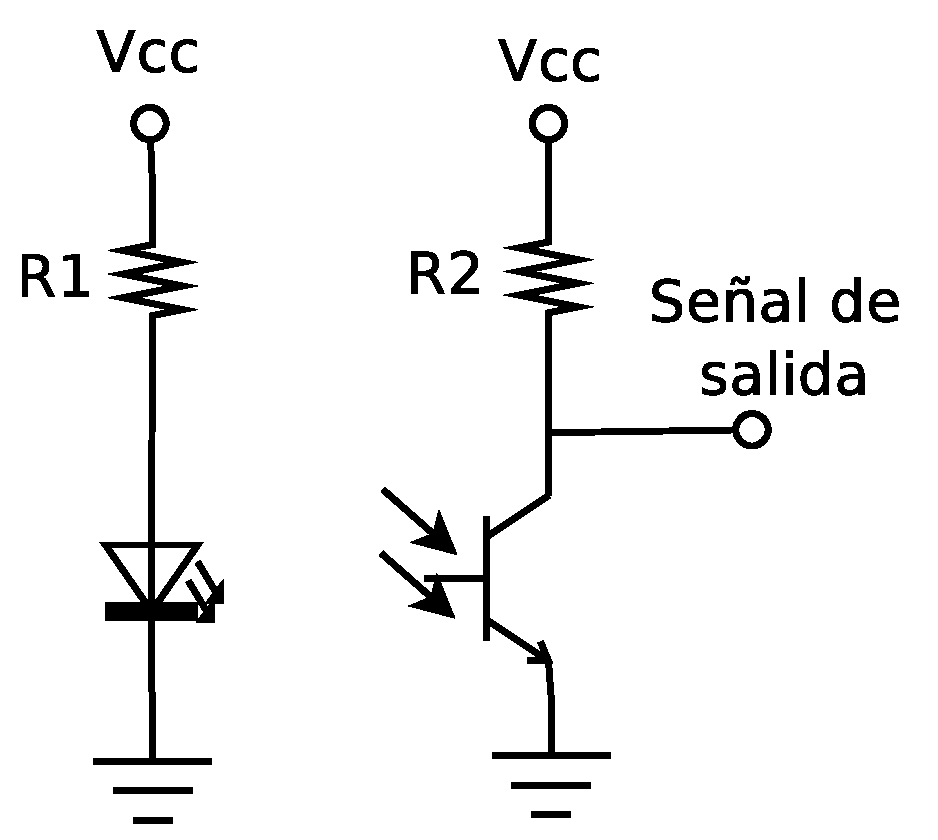
\includegraphics[width=0.3\textwidth]{Figures/Infrarrojo.eps}
  \caption{Circuito emisor-receptor IR.}
  \label{fig:CircuitoIR}
\end{figure}

\end{document}

%%% Local Variables:
%%% mode: latex
%%% TeX-master: t
%%% End:
